\documentclass[border=3pt,tikz]{standalone}
% Shared look for every TikZ figure in these notes.
% Included by each standalone figure file; also keeps the figures consistent
% with the colours used in the PDF and on the website.

\usepackage{tikz}
\usepackage{pgfplots}
\pgfplotsset{compat=1.18}
\usetikzlibrary{arrows.meta, decorations.markings, decorations.pathmorphing,
                patterns, calc, positioning}
\usepackage{amsmath}

% Series colours are the three validated categorical slots also used by the
% interactive widgets, so a path drawn in the printed notes and the same path on
% the website are the same colour. They clear the colour-vision-deficiency and
% contrast checks as a set; every path is direct-labelled as well, so colour is
% never the only thing carrying identity.
\definecolor{duPurple}{HTML}{68246D}
\definecolor{duBlue}{HTML}{2A78D6}
\definecolor{duRed}{HTML}{EB6834}
\definecolor{duGreen}{HTML}{1BAF7A}
\definecolor{duGrey}{HTML}{4D4D4D}

\tikzset{
  % heavier default lines and arrow tips, so diagrams stay clear when zoomed
  every picture/.append style = {line width=0.7pt, >={Stealth[length=3mm]}},
  axisline/.style   = {-{Stealth[length=3.4mm]}, line width=1.0pt, black},
  path1/.style      = {duBlue,   line width=1.6pt},
  path2/.style      = {duRed,    line width=1.6pt},
  path3/.style      = {duGreen,  line width=1.6pt},
  statedot/.style   = {circle, fill=black, inner sep=1.8pt},
  arrowhead/.style  = {decoration={markings,
                        mark=at position #1 with {\arrow{Stealth[length=3.4mm]}}},
                       postaction={decorate}},
  lbl/.style        = {font=\normalsize},
  slbl/.style       = {font=\small, duGrey},
  workfill/.style   = {duPurple, opacity=0.16},
}

% larger labels in plots as well
\pgfplotsset{every axis/.append style={label style={font=\normalsize}, tick label style={font=\small}, line width=0.9pt}}

% Compression by an external force: the piston (area A) is about to move a
% distance dl into the gas (dashed line), sweeping out the hatched volume dV.
\begin{document}
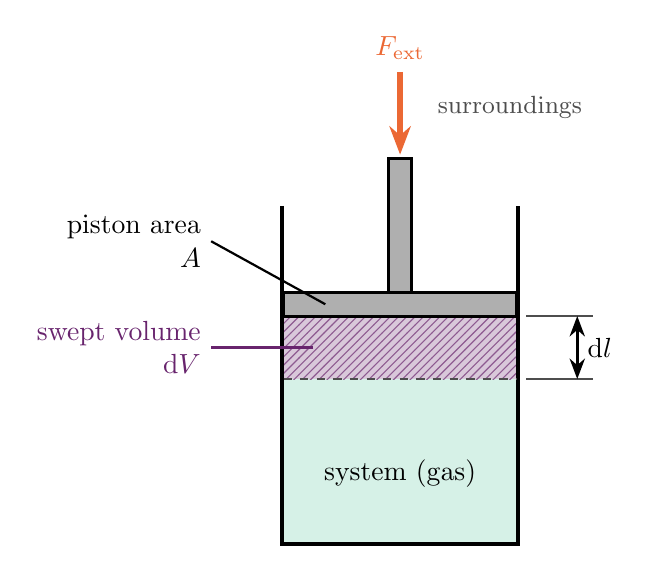
\begin{tikzpicture}[x=1cm, y=1cm]
  \def\W{3.0}      % cylinder inner width
  \def\yo{2.9}     % piston (bottom face) before
  \def\yn{2.1}     % piston (bottom face) after
  \def\t{0.3}      % piston thickness
  % ---- gas (system) ------------------------------------------------------
  \fill[duGreen!18] (0,0) rectangle (\W,\yo);
  % ---- swept volume dV: the slab the piston moves through -----------------
  \fill[duPurple!25] (0,\yn) rectangle (\W,\yo);
  \fill[pattern=north east lines, pattern color=duPurple!75] (0,\yn) rectangle (\W,\yo);
  % ---- cylinder walls ----------------------------------------------------
  \draw[line width=1.4pt] (0,4.3) -- (0,0) -- (\W,0) -- (\W,4.3);
  % ---- piston now (solid) and a moment later (dashed) ---------------------
  \fill[duGrey!45] (0.02,\yo) rectangle (\W-0.02,\yo+\t);
  \draw[line width=1.1pt] (0.02,\yo) rectangle (\W-0.02,\yo+\t);
  \draw[duGrey, dashed, line width=1pt] (0.02,\yn) -- (\W-0.02,\yn);
  \fill[duGrey!45] (\W/2-0.15,\yo+\t) rectangle (\W/2+0.15,4.9);
  \draw[line width=1.1pt] (\W/2-0.15,\yo+\t) rectangle (\W/2+0.15,4.9);
  % ---- external force ----------------------------------------------------
  \draw[-{Stealth[length=3.6mm]}, line width=2pt, duRed] (\W/2,6.0) -- (\W/2,4.95)
    node[pos=0, above, font=\normalsize] {$F_\text{ext}$};
  % ---- dl: how far the piston moves --------------------------------------
  \draw[duGrey, line width=0.6pt] (\W+0.1,\yo) -- (\W+0.95,\yo);
  \draw[duGrey, line width=0.6pt] (\W+0.1,\yn) -- (\W+0.95,\yn);
  \draw[{Stealth[length=2.6mm]}-{Stealth[length=2.6mm]}, line width=0.9pt]
    (\W+0.75,\yn) -- (\W+0.75,\yo) node[midway, right, font=\normalsize] {$\mathrm{d}l$};
  % ---- dV: the swept volume ----------------------------------------------
  \draw[duPurple, line width=0.8pt] (0.4,{(\yn+\yo)/2}) -- (-0.9,{(\yn+\yo)/2})
    node[left, font=\normalsize, text=duPurple, align=right] {swept volume\\$\mathrm{d}V$};
  % ---- A: the piston area ------------------------------------------------
  \draw[line width=0.8pt] (0.55,\yo+0.15) -- (-0.9,\yo+0.95)
    node[left, font=\normalsize, align=right] {piston area\\$A$};
  % ---- labels --------------------------------------------------------------
  \node[font=\normalsize] at (\W/2,0.9) {system (gas)};
  \node[slbl, anchor=west] at (\W/2+0.35,5.55) {surroundings};
\end{tikzpicture}
\end{document}
